\documentclass{article}
\usepackage[utf8]{inputenc}
\usepackage[spanish]{babel}
\usepackage{graphicx}
\graphicspath{ {images/} }

\begin{document}

\begin{titlepage}
    \begin{center}
        \vspace*{1cm}
            
        \Huge
        \textbf{Analisis}
            
        \vspace{0.5cm}
        \LARGE
        Parcial 2
            
        \vspace{1.5cm}
            
        \textbf{Danier Santiago Ortega Restrepo}
            
        \vfill
            
        \vspace{0.8cm}
            
        \Large
        Despartamento de Ingeniería Electrónica y Telecomunicaciones\\
        Universidad de Antioquia\\
        Medellín\\
       Septiembre de 2021
            
    \end{center}
\end{titlepage}

\newpage
\tableofcontents
\section{RECURSOS}
Despues de leer las indicaciones del parcial 2, primero se tendran en cuenta los recursos disponibles para la realizacion de este, se estudiaran conceptos de manejo de leds RGB(red green and blue), uso de la plataforma Tinkercad, arduino, lenguaje C++, informacion multimedia relacionada con el proyecto y enfasis en el tiempo de realizacion.

Algunos recursos probables pero de analizar, circuito integrado, entorno de desarrollo arduino, ya sea online o descargar la app, 

\section{PROPUESTA}
Una propuesta para empezar el parcial seria empezar por practicar con algunos leds RGB y practicar su funcionamiento y asi practicar su funcionamiendo y maniobrabilidad de colores a conveniencia del usuario.

Practicar el procesamiento de imagenes dictado por el profesor y buscar ayudas para la implementacion de esta parte fundamental, ya que a partir de el manejo adecuado de la imagen dependera la adaptacion a el arreglo de leds.

Crear funciones para lectura de imagen, adaptacion de imagen para el tamaño 8x8 sin importar la dimension de la imagen agregada, implementar una clase que trabaje con los pixeles que contega la imagen y retorne bits para implementarlos en la placa arduino y trasmitirlos a los leds 8x8.

Adaptar el codigo c++ trabajado en Qt al arduino y sus condiciones, ademas de tener en cuenta el tamaño de las variables para evitar lentitud en el procesamiento de las imagenes.

Leer archivos PNG en Qt, para esto se debe investigar como se trabaja la lectura y organizar estos datos de salida de tal forma que se puedan ingresar a la placa de arduino por las entradas seriales.

Crear la matriz de leds e implementar un metodo de organizacion de tal forma que se pueda trabajar con cada uno  de los leds de manera acertada, verificar metodos de submuestreo y sobremuestreo para las imagenes, estudiar algoritmos de estos metodos ateriormente mencionados.

\section{IDEA}
En la imagen siguiente vemos una idea de partida para el parcial en donde se trabaja desde la parte en que se ingresan los datos a la placa de arduino para su posterior funcionamiento.\\
    \begin{figure}[h]
    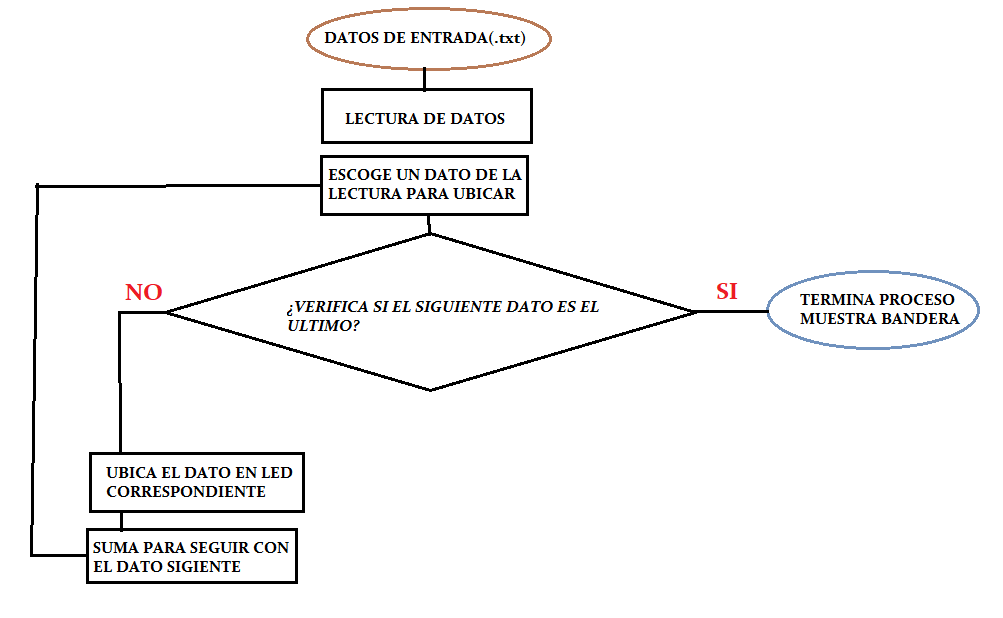
\includegraphics[width=13cm]{diagrama.png}
    \centering
    \caption{Diagrama de idea general}
    \label{fig:diagrama}
    \end{figure}




\bibliographystyle{IEEEtran}
\bibliography{references}
\end{document}
